%&LaTeX
\documentclass[11pt]{article}


% keep the following two lines; makes very nice pdf files when using ps2pdf
\usepackage[T1]{fontenc}
\usepackage{ae,aecompl}

\usepackage[normalem]{ulem}
\usepackage{fullpage}
\usepackage{setspace}
\usepackage{type1cm} % computer modern fonts
\usepackage{fancyhdr}
\usepackage{natbib}
%\usepackage[sort]{natbib}
%\usepackage{epsfig,psfrag,amsmath,amssymb,subfigure,setspace,rotating}
\usepackage{graphicx,psfrag,amsmath,amssymb,subfigure,setspace,rotating}

\usepackage{enumitem}

\usepackage[perpage,para,symbol]{footmisc}

\usepackage[usenames]{color}  % allows colored text

%\usepackage[sort]{natbib}
%\usepackage{epsfig,psfrag,amsmath,amssymb,subfigure}

% Mike's new commands \comm and \kill: uncomment if you want to use
\newcommand{\comm}[1]{\textcolor{blue}{\textit{#1}}}
\renewcommand{\kill}[1]{\textcolor{red}{\sout{#1}}}

\setlength{\parindent}{0.in}
\setlength{\parskip}{0.1in}

\newenvironment{itemize*}%
{\begin{itemize}[label=\textbullet,leftmargin=1pc,labelsep=*,noitemsep,
topsep=0.3pc,parsep=0.4pc]}
 {\end{itemize}}


%\pagestyle{fancy}
%\lhead{Wind-Turbine Structural Dynamics}
%\chead{}
%\rhead{2011 LDRD Proposal}




% \textheight=10.0in


\newcommand{\ie}{\textit{i.e.},~}
\newcommand{\eg}{\textit{e.g.},~}
\newcommand{\bs}{\boldsymbol}
\newcommand{\Ss}{\scriptscriptstyle}
\newcommand{\D}{\mathrm{d}}

\begin{document}  


\section*{Proposed geometric entities and data structures for code coupling
in FAST}

Michael A. Sprague \& John Michalakes, Draft, 7 December 2011

\section{Motivation, goals, notes}

\begin{itemize}

\item This document is towards defining an appropriate coupling framework
for FAST and FAST-related programs.  

\item A motivation is to provide consistent guidance to developers to
provide interface data in a standardized manner that simplifies coupling
with other components.

\item Any framework must general enough to explore/incorporate various
algorithmic coupling approaches.

\end{itemize}

\section{Geometric entities for coupling}

We assume that the ``physical'' interface of a component is either one of
the following or some combination:

\begin{enumerate} 
\item a point  (\eg  connection of a mooring line)

\item a line (may be curved) (\eg a beam representation of a blade)

\item a surface (\eg pressure distribution over a blade)

\item a volume (\eg OpenFOAM finite volume)

\end{enumerate}

These four geometric entities can be well described in a standard
isoparametric mapping, which is closely related to the finite-element
method; see Figs. 1-3.  

The elements and numbering schemes shown in Figs. 1-3 define unique
interpolation.  The inclusion of midside nodes allows for unique
representation of curved line/surface with quadratic polynomials.  The
elements shown in Figs. 1-3 are standard elements, and are available in most
meshing software.


\textbf{Remark:} Using a finite-element representation of component
interfaces has nothing to do with the discretization used by the underlying
components.

Interface elements:

Point: point

Line (Fig. 1): two-node (linear) or three-node (quadratic) line elements

Surface (Fig. 2): 3-node \& 6-node triangles elements; 4-node \& 8-node 
quadrilateral elements

Volume (Fig. 3): 8-node \& 20-node hexahedral elements;  
6-node \& 15-node wedge-elements;
4-node \& 10-node tetrahedron elements

\textbf{Remarks:} Figs. 1-3 show a standard numbering scheme. Linear-element 
numbering is a subset of the quadratic-element numbering shown.  For
example, a linear quadrilateral is defined just by the corner nodes, 1--4.

\section{Coupling-interface data structures}

Here we assume we have a model where we know global position coordinates at
each "node" along with one or more number of degrees of freedom that are
known at each node.   In this description, we consider a single degree of
freedom, say displacement $u$.  Other degrees of freedom might by
temperature, rotation, local coordinates, etc.  Further, in addition to
scalar quantities, we could pass  vector, or tensor quantities.

\textbf{Approach:}\\
Assume that we have $N$ nodes on the boundary of the domain associated with
one code.  
Provide all boundary data as a $N$-dimensional real/double-precision arrays,
including global data positions and degrees of freedom (here $u$); 
\begin{verbatim}
integer N                    ! number of boundary nodes
double precision  xyz(N,3)   ! global xyz coordinates on bndry
double precision  u(N)       ! u response on bndry
\end{verbatim}

Create integer arrays that describe how the above boundary nodes are
connected, using elements described above:
\begin{verbatim}
integer Npoint               ! number of point elements
integer Nline2               ! number of 2-node line elements
integer Nline3               ! number of 3-node line elements
integer Ntri3                ! number of 3-node triangle elements
integer Ntri6                ! number of 6-node triangle elements
integer Nquad4               ! number of 4-node quadrilateral elements
integer Nquad8               ! number of 8-node quadrilateral elements
integer Ntet4                ! number of 4-node tet elements
integer Ntet10               ! number of 10-node tet elements
integer Nhex8                ! number of 8-node hex elements
integer Nhex10               ! number of 20-node hex elements
integer Nwedge6              ! number of 6-node wedge elements
integer Nwedge15             ! number of 15-node wedgeelements

integer element_point(Npoint)        ! point connectivity
integer element_line2(2,Nline2)      ! 2-node line connectivity
integer element_line3(3,Nline3)      ! 3-node line connectivity
integer element_line2(2,Ntri3)       ! 3-node triangle connectivity
integer element_line3(3,Ntri6)       ! 6-node triangle connectivity
integer element_quad4(4,Nquad4)      ! 4-node quad connectivity
integer element_quad8(8,Nquad8)      ! 8-node quad connectivity
integer element_tet4(4,Ntet4)        ! 3-node tet connectivity
integer element_tet10(10,Ntet10)     ! 10-node tet connectivity
integer element_hex8(8,Nhex8)        ! 8-node hex connectivity
integer element_hex20(20,Nhex20)     ! 20-node hex connectivity
integer element_wedge6(6,Nwedge6)    ! 6-node wedge connectivity
integer element_wedge15(15,Nwedge15) ! 15-node wedge connectivity

\end{verbatim}

With the above definition data can be uniquely interpolated from the nodal
values in $u$.

\textbf{Remark:} There is any number of ways that we could store and
transfer the above data.  The chosen form is verbose, but is clear.  We may
want to make it more succinct.  For example, the numbers of various elements
could be placed into a single integer array.  

%
%
%
%
%
%We wish to be able to transfer input-output properties across the coupled
%interface.  This is specific to the "self" domain.  For example, say we have
%a square surface defined by a single 4-node element.  The data required to
%build a coupling routine could be embodied as (\# denotes a comment line).
%Here we assume that output data is available at nodes, and the locations
%required for input data are defined in element-level natural coordinates.
%For example, for the following surface element, we want input forcing/data
%at Gauss points.
%
%\textbf{Remark:} The following is a ``text file'' realization of what could
%easily be a data stream transferred between programs to build up the
%coupling structure.  Following what is shown could be a list of all data
%available at each node, e.g. displacements, locations, etc.
%
%\clearpage
%\begin{verbatim}
%#--------------------------------------------------------------------
%#---------------- nodes  --------------------------------------------
%# number of nodes
%4
%# node number and locations:  num, x, y, z
%1 0. 0. 0.
%2 1. 0. 0.
%3 0. 1. 0.
%4 1. 1. 0.
%#--------------------------------------------------------------------
%#---------------- point elements ------------------------------------
%# number of point elements
%0
%# point-element definitions: number of nodes, n1, n2, ... 
%# number of input-points (None if no elements)
%# surface-element input-points (in element natural coordinates)
%#--------------------------------------------------------------------
%#---------------- line elements -------------------------------------
%# number of line elements
%0
%# line-element definitions: number of nodes, n1, n2, ... 
%# number of input-points (None if no elements)
%# surface-element input-points (in element natural coordinates)
%#--------------------------------------------------------------------
%#---------------- surface elements ----------------------------------
%# number of surface elements
%1
%# surface-element definitions: number of nodes, n1, n2, ... 
%4 1 2 4 3
%# number of input-points (none if no elements)
%4
%# surface-element input-points (in element natural coordinates)
%-0.577 -0.577
% 0.577 -0.577
%-0.577  0.577
% 0.577  0.577 
%#--------------------------------------------------------------------
%#---------------- volume elements -----------------------------------
%# number of volume elements
%0
%# volume-element definitions: number of nodes, n1, n2, ... 
%# number of input-points (None if no elements)
%# surface-element input-points (in element natural coordinates)
%
%\end{verbatim}
%
%
%
%
%
\begin{figure}[h!p]
\centering
     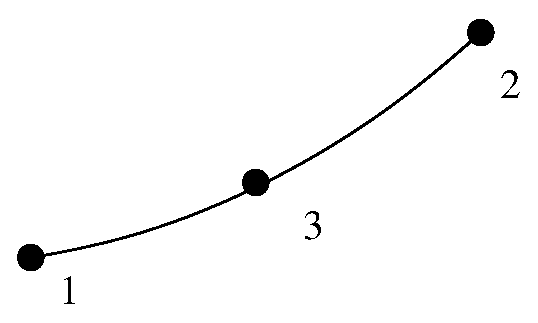
\includegraphics[width=1.8in]{figs/line3.xfig.eps}
     \caption{Element connectivities for line
     elements. Numbering for linear (1--2) and quadratic (1--3) elements are
     shown.}
     \label{el_num}
\end{figure}

\begin{figure}[h!p]
\centering
    \subfigure[]{
     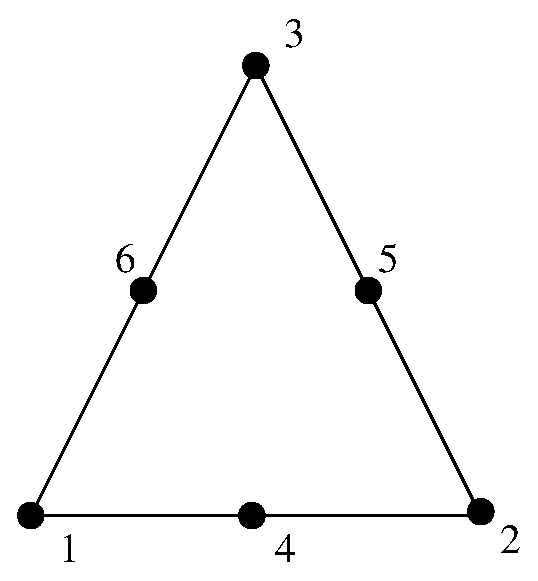
\includegraphics[width=1.8in]{figs/tri6.xfig.eps}} \hspace{0.4in}
     \subfigure[]{
     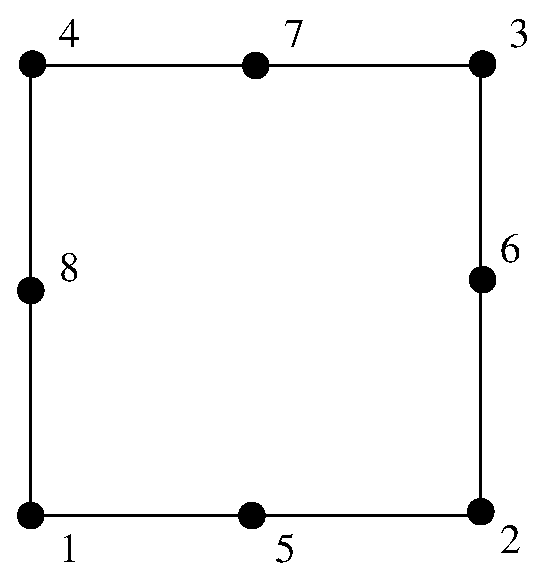
\includegraphics[width=1.8in]{figs/square8.xfig.eps}} \hspace{0.4in}
     \caption{Element connectivities for triangle and square surface
     elements. Numbering for linear and quadratic (serendipity) elements are
     shown.}
     \label{el_num}
\end{figure}


\begin{figure}[h!p]
\centering
    \subfigure[]{
     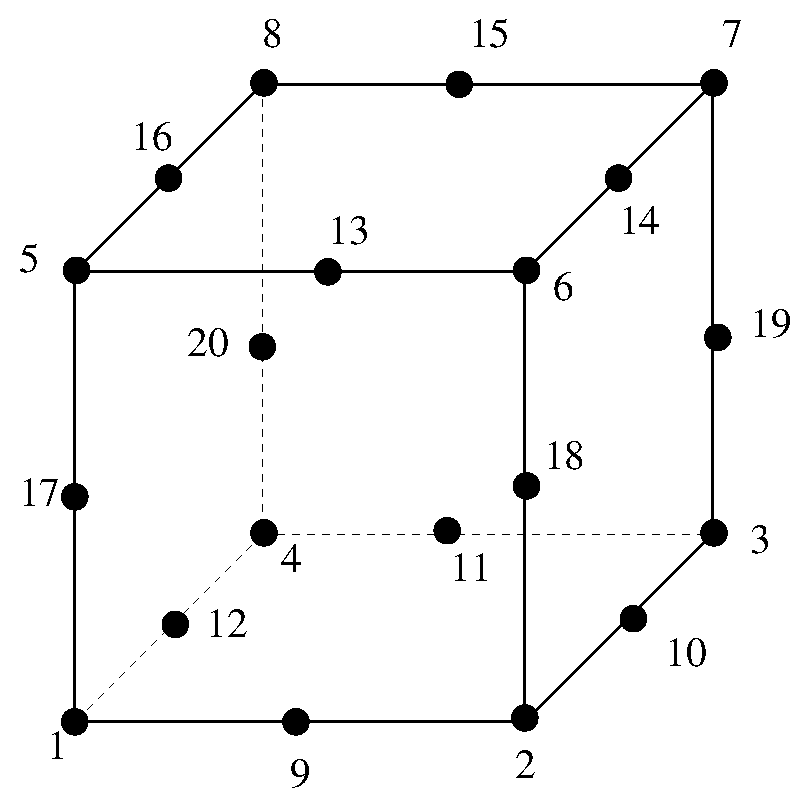
\includegraphics[width=2.5in]{figs/hex.xfig.eps}} \hspace{0.4in}
     \subfigure[]{
     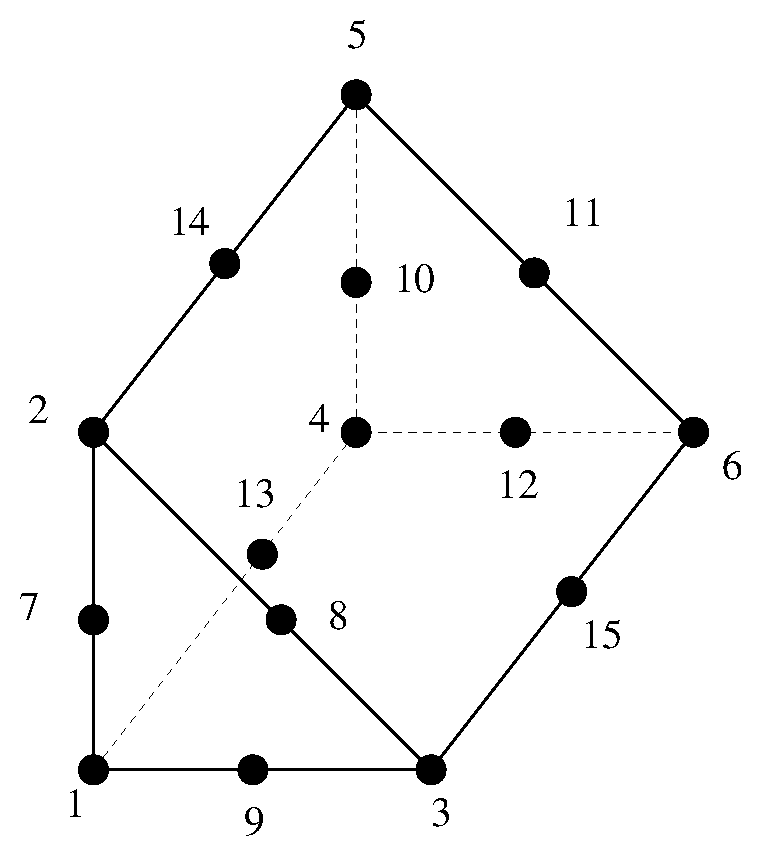
\includegraphics[width=2.5in]{figs/wedge.xfig.eps}} \hspace{0.4in}
     \subfigure[]{
     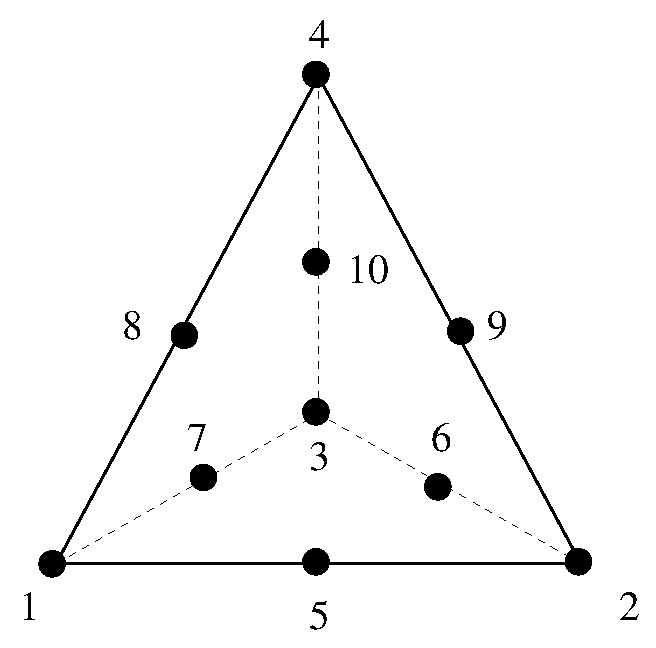
\includegraphics[width=2.5in]{figs/tet.xfig.eps}} \hspace{0.4in}
     \caption{Element connectivities for hexagonal, wedge, and tet
     elements. Numbering for linear and quadratic (serendipity) elements are
     shown.}
     \label{el_num}
\end{figure}




%\bibliography{ref_template}
%\bibliographystyle{jfm}
%\bibliographystyle{chicago}
%\bibliographystyle{plain}

\end{document}  

